
%% bare_conf.tex
%% V1.3
%% 2007/01/11
%% by Michael Shell
%% See:
%% http://www.michaelshell.org/
%% for current contact information.
%%
%% This is a skeleton file demonstrating the use of IEEEtran.cls
%% (requires IEEEtran.cls version 1.7 or later) with an IEEE conference paper.
%% Support sites:
%% http://www.michaelshell.org/tex/ieeetran/
%% http://www.ctan.org/tex-archive/macros/latex/contrib/IEEEtran/
%% and
%% http://www.ieee.org/

%%*************************************************************************
%% Legal Notice:
%% This code is offered as-is without any warranty either expressed or
%% implied; without even the implied warranty of MERCHANTABILITY or
%% FITNESS FOR A PARTICULAR PURPOSE! 
%% User assumes all risk.
%% In no event shall IEEE or any contributor to this code be liable for
%% any damages or losses, including, but not limited to, incidental,
%% consequential, or any other damages, resulting from the use or misuse
%% of any information contained here.
%%
%% All comments are the opinions of their respective authors and are not
%% necessarily endorsed by the IEEE.
%%
%% This work is distributed under the LaTeX Project Public License (LPPL)
%% ( http://www.latex-project.org/ ) version 1.3, and may be freely used,
%% distributed and modified. A copy of the LPPL, version 1.3, is included
%% in the base LaTeX documentation of all distributions of LaTeX released
%% 2003/12/01 or later.
%% Retain all contribution notices and credits.
%% ** Modified files should be clearly indicated as such, including  **
%% ** renaming them and changing author support contact information. **
%%
%% File list of work: IEEEtran.cls, IEEEtran_HOWTO.pdf, bare_adv.tex,
%%                    bare_conf.tex, bare_jrnl.tex, bare_jrnl_compsoc.tex
%%*************************************************************************

% *** Authors should verify (and, if needed, correct) their LaTeX system  ***
% *** with the testflow diagnostic prior to trusting their LaTeX platform ***
% *** with production work. IEEE's font choices can trigger bugs that do  ***
% *** not appear when using other class files.                            ***
% The testflow support page is at:
% http://www.michaelshell.org/tex/testflow/

% Also note that the "draftcls" or "draftclsnofoot", not "draft", option
% should be used if it is desired that the figures are to be displayed in
% draft mode.
%
\documentclass[conference]{IEEEtran}


% Some very useful LaTeX packages include:
% (uncomment the ones you want to load)


% *** MISC UTILITY PACKAGES ***
%
%\usepackage{ifpdf}
% Heiko Oberdiek's ifpdf.sty is very useful if you need conditional
% compilation based on whether the output is pdf or dvi.
% usage:
% \ifpdf
%   % pdf code
% \else
%   % dvi code
% \fi
% The latest version of ifpdf.sty can be obtained from:
% http://www.ctan.org/tex-archive/macros/latex/contrib/oberdiek/
% Also, note that IEEEtran.cls V1.7 and later provides a builtin
% \ifCLASSINFOpdf conditional that works the same way.
% When switching from latex to pdflatex and vice-versa, the compiler may
% have to be run twice to clear warning/error messages.



% *** CITATION PACKAGES ***
\usepackage{cite}
% cite.sty was written by Donald Arseneau
% V1.6 and later of IEEEtran pre-defines the format of the cite.sty package
% \cite{} output to follow that of IEEE. Loading the cite package will
% result in citation numbers being automatically sorted and properly
% "compressed/ranged". e.g., [1], [9], [2], [7], [5], [6] without using
% cite.sty will become [1], [2], [5]--[7], [9] using cite.sty. cite.sty's
% \cite will automatically add leading space, if needed. Use cite.sty's
% noadjust option (cite.sty V3.8 and later) if you want to turn this off.
% cite.sty is already installed on most LaTeX systems. Be sure and use
% version 4.0 (2003-05-27) and later if using hyperref.sty. cite.sty does
% not currently provide for hyperlinked citations.
% The latest version can be obtained at:
% http://www.ctan.org/tex-archive/macros/latex/contrib/cite/
% The documentation is contained in the cite.sty file itself.



% *** GRAPHICS RELATED PACKAGES ***
%
\ifCLASSINFOpdf
  \usepackage[pdftex]{graphicx}
  % declare the path(s) where your graphic files are
  % \graphicspath{{../pdf/}{../jpeg/}}
  % and their extensions so you won't have to specify these with
  % every instance of \includegraphics
  % \DeclareGraphicsExtensions{.pdf,.jpeg,.png}
\else
  % or other class option (dvipsone, dvipdf, if not using dvips). graphicx
  % will default to the driver specified in the system graphics.cfg if no
  % driver is specified.
  % \usepackage[dvips]{graphicx}
  % declare the path(s) where your graphic files are
  % \graphicspath{{../eps/}}
  % and their extensions so you won't have to specify these with
  % every instance of \includegraphics
  % \DeclareGraphicsExtensions{.eps}
\fi


% *** MATH PACKAGES ***
%
%\usepackage[cmex10]{amsmath}
% A popular package from the American Mathematical Society that provides
% many useful and powerful commands for dealing with mathematics. If using
% it, be sure to load this package with the cmex10 option to ensure that
% only type 1 fonts will utilized at all point sizes. Without this option,
% it is possible that some math symbols, particularly those within
% footnotes, will be rendered in bitmap form which will result in a
% document that can not be IEEE Xplore compliant!
%
% Also, note that the amsmath package sets \interdisplaylinepenalty to 10000
% thus preventing page breaks from occurring within multiline equations. Use:
%\interdisplaylinepenalty=2500
% after loading amsmath to restore such page breaks as IEEEtran.cls normally
% does. amsmath.sty is already installed on most LaTeX systems. The latest
% version and documentation can be obtained at:
% http://www.ctan.org/tex-archive/macros/latex/required/amslatex/math/



% *** SPECIALIZED LIST PACKAGES ***
%
%\usepackage{algorithmic}
% algorithmic.sty was written by Peter Williams and Rogerio Brito.
% This package provides an algorithmic environment fo describing algorithms.
% You can use the algorithmic environment in-text or within a figure
% environment to provide for a floating algorithm. Do NOT use the algorithm
% floating environment provided by algorithm.sty (by the same authors) or
% algorithm2e.sty (by Christophe Fiorio) as IEEE does not use dedicated
% algorithm float types and packages that provide these will not provide
% correct IEEE style captions. The latest version and documentation of
% algorithmic.sty can be obtained at:
% http://www.ctan.org/tex-archive/macros/latex/contrib/algorithms/
% There is also a support site at:
% http://algorithms.berlios.de/index.html
% Also of interest may be the (relatively newer and more customizable)
% algorithmicx.sty package by Szasz Janos:
% http://www.ctan.org/tex-archive/macros/latex/contrib/algorithmicx/



% *** ALIGNMENT PACKAGES ***
%
%\usepackage{array}
% Frank Mittelbach's and David Carlisle's array.sty patches and improves
% the standard LaTeX2e array and tabular environments to provide better
% appearance and additional user controls. As the default LaTeX2e table
% generation code is lacking to the point of almost being broken with
% respect to the quality of the end results, all users are strongly
% advised to use an enhanced (at the very least that provided by array.sty)
% set of table tools. array.sty is already installed on most systems. The
% latest version and documentation can be obtained at:
% http://www.ctan.org/tex-archive/macros/latex/required/tools/


%\usepackage{mdwmath}
%\usepackage{mdwtab}
% Also highly recommended is Mark Wooding's extremely powerful MDW tools,
% especially mdwmath.sty and mdwtab.sty which are used to format equations
% and tables, respectively. The MDWtools set is already installed on most
% LaTeX systems. The lastest version and documentation is available at:
% http://www.ctan.org/tex-archive/macros/latex/contrib/mdwtools/


% IEEEtran contains the IEEEeqnarray family of commands that can be used to
% generate multiline equations as well as matrices, tables, etc., of high
% quality.


%\usepackage{eqparbox}
% Also of notable interest is Scott Pakin's eqparbox package for creating
% (automatically sized) equal width boxes - aka "natural width parboxes".
% Available at:
% http://www.ctan.org/tex-archive/macros/latex/contrib/eqparbox/


% *** SUBFIGURE PACKAGES ***
%\usepackage[tight,footnotesize]{subfigure}
% subfigure.sty was written by Steven Douglas Cochran. This package makes it
% easy to put subfigures in your figures. e.g., "Figure 1a and 1b". For IEEE
% work, it is a good idea to load it with the tight package option to reduce
% the amount of white space around the subfigures. subfigure.sty is already
% installed on most LaTeX systems. The latest version and documentation can
% be obtained at:
% http://www.ctan.org/tex-archive/obsolete/macros/latex/contrib/subfigure/
% subfigure.sty has been superceeded by subfig.sty.



%\usepackage[caption=false]{caption}
%\usepackage[font=footnotesize]{subfig}
% subfig.sty, also written by Steven Douglas Cochran, is the modern
% replacement for subfigure.sty. However, subfig.sty requires and
% automatically loads Axel Sommerfeldt's caption.sty which will override
% IEEEtran.cls handling of captions and this will result in nonIEEE style
% figure/table captions. To prevent this problem, be sure and preload
% caption.sty with its "caption=false" package option. This is will preserve
% IEEEtran.cls handing of captions. Version 1.3 (2005/06/28) and later 
% (recommended due to many improvements over 1.2) of subfig.sty supports
% the caption=false option directly:
%\usepackage[caption=false,font=footnotesize]{subfig}
%
% The latest version and documentation can be obtained at:
% http://www.ctan.org/tex-archive/macros/latex/contrib/subfig/
% The latest version and documentation of caption.sty can be obtained at:
% http://www.ctan.org/tex-archive/macros/latex/contrib/caption/




% *** FLOAT PACKAGES ***
%
%\usepackage{fixltx2e}
% fixltx2e, the successor to the earlier fix2col.sty, was written by
% Frank Mittelbach and David Carlisle. This package corrects a few problems
% in the LaTeX2e kernel, the most notable of which is that in current
% LaTeX2e releases, the ordering of single and double column floats is not
% guaranteed to be preserved. Thus, an unpatched LaTeX2e can allow a
% single column figure to be placed prior to an earlier double column
% figure. The latest version and documentation can be found at:
% http://www.ctan.org/tex-archive/macros/latex/base/



%\usepackage{stfloats}
% stfloats.sty was written by Sigitas Tolusis. This package gives LaTeX2e
% the ability to do double column floats at the bottom of the page as well
% as the top. (e.g., "\begin{figure*}[!b]" is not normally possible in
% LaTeX2e). It also provides a command:
%\fnbelowfloat
% to enable the placement of footnotes below bottom floats (the standard
% LaTeX2e kernel puts them above bottom floats). This is an invasive package
% which rewrites many portions of the LaTeX2e float routines. It may not work
% with other packages that modify the LaTeX2e float routines. The latest
% version and documentation can be obtained at:
% http://www.ctan.org/tex-archive/macros/latex/contrib/sttools/
% Documentation is contained in the stfloats.sty comments as well as in the
% presfull.pdf file. Do not use the stfloats baselinefloat ability as IEEE
% does not allow \baselineskip to stretch. Authors submitting work to the
% IEEE should note that IEEE rarely uses double column equations and
% that authors should try to avoid such use. Do not be tempted to use the
% cuted.sty or midfloat.sty packages (also by Sigitas Tolusis) as IEEE does
% not format its papers in such ways.



% *** PDF, URL AND HYPERLINK PACKAGES ***
\usepackage{url}
% \url{my_url_here}.


% *** Do not adjust lengths that control margins, column widths, etc. ***
% *** Do not use packages that alter fonts (such as pslatex).         ***
% There should be no need to do such things with IEEEtran.cls V1.6 and later.
% (Unless specifically asked to do so by the journal or conference you plan
% to submit to, of course. )

% allow non-ascii characters
\usepackage[utf8]{inputenc}


% correct bad hyphenation here
\hyphenation{op-tical net-works semi-conduc-tor}


\begin{document}
%
% paper title
% can use linebreaks \\ within to get better formatting as desired
\title{Birmingham Autonomous Robot Club (BARC) - Team Description Paper}


\author{\IEEEauthorblockN{Lenka Mudrova, Marco Becerra, Manolis Chiou, Sean Bastable}
\IEEEauthorblockA{
\{lxm210, mab303, e.chiou, sdb123\}@cs.bham.ac.uk\\
School of Computer Science, University of Birmingham, UK\\
Website: \textit{http://www.cs.bham.ac.uk/$\sim$lxm210/barc.html}}
%\and
%\IEEEauthorblockN{Ashish Kumar}
%\IEEEauthorblockA{axk380@cs.bham.ac.uk}
%\and
%\IEEEauthorblockN{}
%\IEEEauthorblockA{@cs.bham.ac.uk}
}

% conference papers do not typically use \thanks and this command
% is locked out in conference mode. If really needed, such as for
% the acknowledgment of grants, issue a \IEEEoverridecommandlockouts
% after \documentclass

% for over three affiliations, or if they all won't fit within the width
% of the page, use this alternative format:
% 
%\author{\IEEEauthorblockN{Michael Shell\IEEEauthorrefmark{1},
%Homer Simpson\IEEEauthorrefmark{2},
%James Kirk\IEEEauthorrefmark{3}, 
%Montgomery Scott\IEEEauthorrefmark{3} and
%Eldon Tyrell\IEEEauthorrefmark{4}}
%\IEEEauthorblockA{\IEEEauthorrefmark{1}School of Electrical and Computer Engineering\\
%Georgia Institute of Technology,
%Atlanta, Georgia 30332--0250\\ Email: see http://www.michaelshell.org/contact.html}
%\IEEEauthorblockA{\IEEEauthorrefmark{2}Twentieth Century Fox, Springfield, USA\\
%Email: homer@thesimpsons.com}
%\IEEEauthorblockA{\IEEEauthorrefmark{3}Starfleet Academy, San Francisco, California 96678-2391\\
%Telephone: (800) 555--1212, Fax: (888) 555--1212}
%\IEEEauthorblockA{\IEEEauthorrefmark{4}Tyrell Inc., 123 Replicant Street, Los Angeles, California 90210--4321}}


% use for special paper notices
%\IEEEspecialpapernotice{(Invited Paper)}




% make the title area
\maketitle

\begin{abstract}

Birmingham Autonomous Robot Club (BARC) connects students from the School of Computer Science, University of Birmingham, with a strong motivation in robotic applications and competitions. This paper is part of our application for participating in the RoCKIn@Home 2014 competition. It overviews how this challenge relates to our interests and experiences and how we can achieve high reusability of our system by integrating different subsystems from other projects. Moreover, team members, their experiences and research interests are described in detail. This is followed by introducing our robot, its hardware and capabilities. Our intended software structure is also described here, followed by an explanation of the first pilot robotic system, which fulfils a part of the \textit{Welcoming visitors} task. Finally, the conclusion summarises our motivation and relevance for this competition.


\end{abstract}
% IEEEtran.cls defaults to using nonbold math in the Abstract.
% This preserves the distinction between vectors and scalars. However,
% if the conference you are submitting to favors bold math in the abstract,
% then you can use LaTeX's standard command \boldmath at the very start
% of the abstract to achieve this. Many IEEE journals/conferences frown on
% math in the abstract anyway.

% no keywords




% For peer review papers, you can put extra information on the cover
% page as needed:
% \ifCLASSOPTIONpeerreview
% \begin{center} \bfseries EDICS Category: 3-BBND \end{center}
% \fi
%
% For peerreview papers, this IEEEtran command inserts a page break and
% creates the second title. It will be ignored for other modes.
\IEEEpeerreviewmaketitle



\section{Introduction}
% no \IEEEPARstart

Birmingham Autonomous Robot Club (BARC) was established five years ago in the School of Computer Science at the University of Birmingham. The main purpose was to provide an extra opportunity for students to gain additional knowledge about robotics and to work on real robotic platforms and projects. Students were familiarising themselves with the Robot Operating System (ROS) by using a variety of ROS libraries and packages.

Several students involved in the team were contributing to more complicated projects, which were mainly used to promote robotics during the school's open days. Such an example was a robot waitress, which accepted orders for drinks and brought them to the person. This robot had no manipulation, drinks were placed on the robot by a person. Another example is a project using a Nao robot to repeat kids' gestures. An extra Kinect sensor was used to recognise the gestures. In spite of these interesting projects, a lot of students involved in previous years in the club had no real goal and no real deadlines, thus they did not produce any comprehensive work.

This year, the BARC structure was changed in order to incorporate the lessons learned and to allow the team to take part in a robotics competition. We would like to join the RoCKIn@home 2014 competition because it provides an interesting challenge and will help with progressing research and developing applications for domestic and industrial robots. Moreover, the cooperation between students in the team is necessary. As a result, students can learn how to work in a team, but still work on some challenging parts alone and gain valuable knowledge while learning how to be responsible for their work.

The team has the support of the Intelligent Robotics Lab \cite{irlab} in the School of Computer Science. The lab conducts research and has expertise in a variety of fields including but not limited to computer vision, manipulation, planning, architectures, reasoning and mobile robots. Furthermore, the lab has strong links with the industry. 

 
\section{Our focus and plan}

% % % TODO % % % %
%from rules: Innovative technology (if any) TODO describe usage of STRANDS
%from rules: Reusability of the system or parts thereof - see STRANDS
This section summarises three different RoCKIN@home 2014 competition challenges and it describes what is intended to be performed with our robot this year. Our intention is to prepare a complete robotic platform, which will integrate the state of the art in different Artificial Intelligent (AI) areas. The team does not have explicit expertise in any of those fields. Therefore, we would like to aim for high reusability of code in our robotic system and to demonstrate that the current state of the art in AI algorithms can be successfully used to produce a robust, effective and complete robotic system with domestic applications.  

\subsection{Catering for Granny Annie’s Comfort}

A robot will receive requirements from Granny Annie, which may contain interaction with an intelligent flat or bringing to her a specific object. We would like to prepare our robot so that it can perform the first part - cooperation/interaction with an intelligent flat. This subtask still contains interesting challenges, such as robust speech recognition and robot navigation in a way, which is comfortable and natural for a human.  

The problem of speech recognition is often discussed within the robotic community. It is something, which is necessary for future robots to cooperate with humans. Assuming a robot is working at Granny's flat, the robot can learn and adapt to her voice, which will increases its performance over time. Moreover, Granny is living alone, thus, it can be assumed that the level of background noise is minimal. In contrast, during the competition, speech recognition provides a lot of challenges. The background noise is really high during competition because of the spectators. Furthermore, the person playing Granny Annie changes, hence a robot cannot improve its behaviour. We do not plan to develop our system from scratch, rather we plan to use CMU Sphinx - Open Source Toolkit For Speech Recognition \cite{cmu}. 
Moreover, we might cooperate with a Natural Language Processing group within our school to improve the system's behaviour.

For a challenge, where the robot approaches humans, we will use the opportunity for closer cooperation with the STRANDS \cite{strands} project, as our robotics group within our school leads this project. Especially, a cooperation with Christian Dondrup, a PhD student at the University of Lincoln, might be beneficial in this stage, as he is working on Human Robot Interaction.

The second part of this task - bringing someone a specific object - is even more challenging as it includes two large robotics domains, computer vision and manipulation. As our robot has no manipulator this year (see Section \ref{sec:hardware}), we might be able to perform only object search. We might benefit from experiences from a previous project in our robotic group - CogX \cite{cogx}. In this project, one of the robot's abilities was to search for known objects by taking into account common sense knowledge (i.e. prior knowledge) in the form of probabilities of objects' presence in different rooms. However, this will still require a lot of effort from us, as the robot was not using ROS before and we will need to understand and integrate bits into our system. We assume to work on this part next year.

\subsection{Welcoming visitors}

In this task, a robot should welcome visitors, recognize them and accompany them to a specific location in Granny's flat. Several areas are needed in this task: computer vision for face recognition (in the known person case, Dr. Kimbley) and for uniform detection (in the case of the delivery-man). Moreover, machine learning techniques are needed to be able to learn these two patterns in order to recognise them. A robot can also benefit from speech recognition if face/uniform recognition does not provide a certain decision. Finally, a robot must have robust navigation in an environment in order to accompany a person to a specific place. 

In our team, we agreed to start with this task because of our expertise. We have already prepared a robotic system, which is able to recognise faces based on OpenCV (for details see Section \ref{sec:vision}) and robustly navigate in a known environment (see Section \ref{sec:navig}). As a next step, we will work on uniform detection. Again, we will use the expertise within the STRANDS project, where a robot also must recognise different types of uniforms. We also plan to improve the robot's behaviour and we are currently recruiting members towards this goal. For example, it will recognise if a person is following it and will perform actions to ensure this.

\subsection{Getting to know my home}

A robot should recognise changes in a flat in this scenario, which can be done autonomously or by cooperation with a human. It is assumed that our robot will be able to recognise the state of doors autonomously. It will combine measurements taken by a laser scanner and a Kinect. The team has experience with such a problem, thus the already found solution will be integrated into our robotic system. 

In order to automatically recognise changes in the position of furniture or objects, we might take benefit of cooperation with the STRANDS project again, as this is one of the challenges being solved there. However, we plan to combine it with cooperation with a human, where he/she will guide the robot to the object, which has changed position. The algorithms for the robot to be able to follow a person are already prepared. Furthermore, a former team member was working on a project where a robot can recognise where a human finger is pointing. We will use this work and extend it to fit our needs.

\subsection{Timetable}

Our plan is to perform complete \textit{Welcoming visitor}(referred as MW) task during competition. Moreover, we will work on \textit{Getting to know my home}(referred as MG) task, where we assume to be able to recognise state of doors. In order to achieve these goals, we set up our milestones:
\begin{itemize}
\item MW1 - training of a face, recognising a known person based on the face, mapping, localisation, robust navigation in a known map. Deadline: 7.5.2014
\item MW2 - Increase robustness of face recognition, detection if a person is following the robot, speech recognition. Deadline: 27.7.2014
\item MW3 - Integration and test, producing new video. Deadline: 31.7.2014
\item MW4 - Cloth recognition, robot behaviour to restrict person to follow it. Deadline 31.8.2014
\item MW5 - Integration and test. Deadline: 5.9.2014
\item MW6 - \textbf{Perform complete \textit{Welcoming visitor} task during British science festival 6.9.-11.9.2014}
\item MW7 - Perform more test. Deadline 30.9.2014
\item MG1 - Work on autonomous recognition of state of doors, cooperation with human in detection of other changes. Deadline 31.10.2014
\item Test of overall system. Deadline 23.11.2014
\end{itemize}
The expected timetable of our milestones can be seen in Fig. \ref{fig:plan}.

\begin{figure}[!htb]
\centering
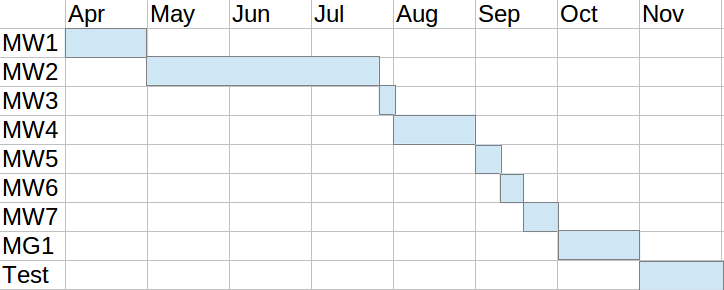
\includegraphics[width=3.in]{timetable.png}
\caption{Timetable}
\label{fig:plan}
\end{figure}



\section{Team members}
%from rules:  Main involved research areas in the team work
Currently, the team has four active members - one bachelor's student and three PhD students in the first year of their studies. All team members are students in the School of Computer Science, University of Birmingham. The overview of team members follows along with a description of their background and research interests. The final team line-up is likely to change before the competition as more members will contribute.

\subsection{Lenka Mudrova}

She is a PhD student with research interests in AI planning and scheduling. In the team, she has two roles. First, she is the team leader, which mainly includes representation of the team when formal communication outside of the team is necessary. Also, she makes sure that every member of the team knows what is happening, how their modules will be used within the system and what is required from them. The second role is that she is working also on the robot's subsystem. Her research interest in Artificial Intelligence (AI) planning will be useful for creating the robot's overall behaviour next year. Moreover, she is interested in computer vision and speech recognition.

\subsubsection*{Scientific background}
She did her bachelor's and master's studies at the Czech Technical University in Prague with a focus on Robotics. This study branch gave her a wide range of knowledge in the fields of mechatronics and artificial intelligence. She was involved as a team leader of the student robotics team FELaaCZech that took part in the international competition Eurobot for four years. 

Currently, she is a PhD student with a focus on AI planning and scheduling, which are important techniques for a robot to make decisions on when, how and what needs to be performed. Such decisions are necessary in service robotics when a robot needs to complete tasks assigned by a human. The robot needs to have a control framework that makes decisions concerning which particular task should be executed. The quality of the decisions influence the overall performance of the robot and of course, the robot's goal must satisfy as many of the requirements assigned by the humans as possible. Requirements for the robot's control framework are deadline awareness, handling uncertainty about task duration and resources, creating plans on how to complete general tasks and awareness of changes in the environment where the robot operates. 

Her research is part of the EU STRANDS project \cite{strands}. "STRANDS aims to enable a robot to achieve robust and intelligent behaviour in human environments through adaptation to, and the exploitation of, long-term experience (at least 120 days by the end of the project).". Therefore, the robot's control framework will exploit long-term experiences and observations of the robot's world. 

\subsection{Marco Antonio Becerra Pedraza}

He is a PhD student in the School of Computer Science, University of Birmingham. His research interests are 3D perception, human sensing, knowledge representation and reasoning. Inside the team he has worked with the human sensing capabilities of the robot.

\subsubsection*{Scientific background}
He obtained his bachelor degree in Mechatronics Engineering from the Instituto Polit\'{e}cnico Nacional in Mexico and a master degree in Computer Science from the Universidad Nacional Aut\'{o}noma de M\'{e}xico. He is a former member of the PUMAS RoboCup@Home team.

During his PhD, he will be doing research about semantic mapping of human events. The topic has two main components:

Semantic mapping can be conceived as an extension of the mapping problem \cite{Nuchter08_TowardsSemanticMaps}. Traditionally maps were used in robotics mostly for navigation purposes. But the environment has additional spatial information that needs to be handled. Semantic maps extend the concept of maps to handle more features from the environment (e.g. structure, functionalities, events). The goal is to reason about the scene (e.g. planning, prediction, explanation, interpretation).

Activity recognition is about using observations from the world to build representations of the ongoing actions. Later, these representations can be used to find associated structures.

\subsection{Manolis Chiou}

He is a PhD student with a multidisciplinary background in control engineering, robotics and AI. His work on BARC involves but is not limited to control, navigation, localisation and in the future Human-Robot-Interaction (HRI).

\subsubsection*{Scientific background}

His first degree is in Control Engineering from the Technological Institute of Piraeus, in which he got involved in a variety of robotic projects including demonstrating these projects to the public and exhibitions. His undergraduate thesis was on implementing control algorithms to robots (e.g. Model Predictive Control for stability/balance). He has an MSc in Computational Intelligence with his master thesis on formation control and transportation of objects with a swarm of robots.  

The working title of his PhD thesis is ``Flexible robotic control via co-operation between an Operator and an AI based control system". It addresses the problem of variable autonomy in teleoperated mobile robots. Variable autonomy refers to the different levels of autonomous capabilities that are implemented on a robot.

Robots used on demanding and safety critical tasks (e.g. search and rescue, hazardous environments inspection, bomb disposal), which are currently teleoperated, could soon start to benefit from autonomous capabilities. Such capabilities include algorithms for automatic robot navigation, algorithms for Simultaneous Localisation And Mapping (SLAM) and etc. Robots could usefully use AI control algorithms to autonomously take control of certain functions when the human operator is suffering a high workload, high cognitive load, anxiety, or other distractions and stresses. In contrast, some circumstances may still necessitate direct human control of the robot. The research will tackle the problem by designing control algorithms for switching between the different autonomy levels in an optimal way. 


\subsection{Sean Bastable}

He is a Computer Science bachelor's student in his final year. It is expected that he will continue to further his studies with a master's degree in Robotics. As the oldest BARC member, he has solid experience with ROS and different robotic platforms. He is also one of the team members who attended RoCKIn camp 2014 in Rome.

\subsubsection*{Scientific background}
 
His final year project was about investigating and implementing a visual localisation system for a mobile robot. This allowed the robot to continue localising in environments where laser based localisation cannot be used. A good example of this is in domestic environments where the presence of people moving around the robot may obstruct the laser scan and provide false readings.
 
The project used a ceiling facing omnidirectional camera on the top of a robot in order to take pictures of its surroundings.
The robot was trained by taking many pictures of the environment, along with location data provided through laser based localisation under ideal conditions. When localising, it can take additional pictures and compare them to the training images in order to find an estimate of its location. Principal Component Analysis (PCA) was used to match images in the localisation phase to those in the test phase. 

Another potential use of this project is to provide an initial location estimate to a laser based localisation system in order to allow the robot to quickly localise from any position without any human input.

This project follows on his previous summer project of a drinks serving robot used in a launch event for the 2014 British Science Festival. As the robot was moving in a crowd, one of the key failure points was that it could become de-localised. The robot had the need to know exactly where it is in order to effectively navigate through gaps in-between crowds. Visual localisation was considered as a potential solution but due to time constrains was not implemented.

\section{\label{sec:hardware}Hardware}
%from rules: Description of the hardware, including an image of the robot(s)
The robot Dora was kindly given for the team's needs, see Fig.\ref{fig:dora}. She is constructed from a Pioneer 3D-X, which is differential wheel robotic platform with a Hokuyo laser scanner mounted on the front. Moreover, a pan-tilt unit carrying a Kinect depth camera and one RGB camera are mounted on the higher point of the platform in order to get snapshots from better views than if they were placed on the Pioneer robot. Dora also has a travel luggage kit, thus it is possible to take her to the competition.

Furthermore, team members have access to different sensors such as laser scanners, depth and RGB cameras. At the moment, Dora has no manipulator arm installed. In the future, it is planned to mount one small manipulator arm in order to extend Dora's capabilities.

\begin{figure}[!t]
\centering
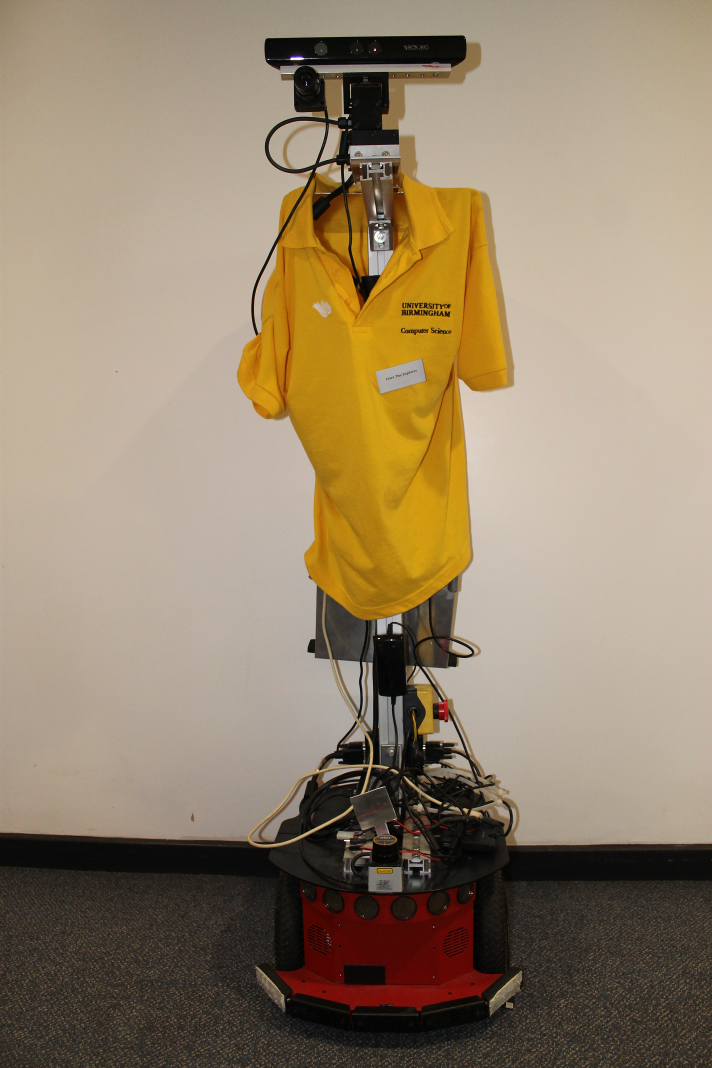
\includegraphics[width=2.in]{dora_new.png}
\caption{Dora is an extended Pioneer 3D-X robot with sensors such as a laser range finder, depth camera and a laptop mounted on top.}
\label{fig:dora}
\end{figure}

\section{Software architecture}

As our goal is to achieve high reusability, modularity and openness, we built our software architecture on the Robot Operating System (ROS) middleware, using version Hydro \cite{ros}. ROS's open source philosophy is powerful and allows code reusability by different programmers. It allows us to use robust, state-of-the-art subsystems which are not in our research interest, such as localisation, mapping and navigation around obstacles. We can even add our own AI algorithms without worrying how to access specific hardware on a robot, as standard drivers are provided by ROS for many items of hardware used in robotics. Even more important is the fact that it provides a standardised way to provide inputs/outputs of subsystems. As a result, it can save valuable time during the merging of different subsystems written by different users. Last but not least, ROS was also chosen as it has become almost a standard choice for researchers.
%and thus our lab has extensive hands on experience.

In order to fulfil the \textit{Welcoming visitors} task, we have already developed some main components such as face recognition and navigation. Moreover, we have created a basic structure of our software system for this task, which links all used components/ROS nodes, see Fig. \ref{fig:nodes}. The different nodes communicate by exchanging ROS messages and by using ROS actions.

\begin{figure*}[!t]
\centering
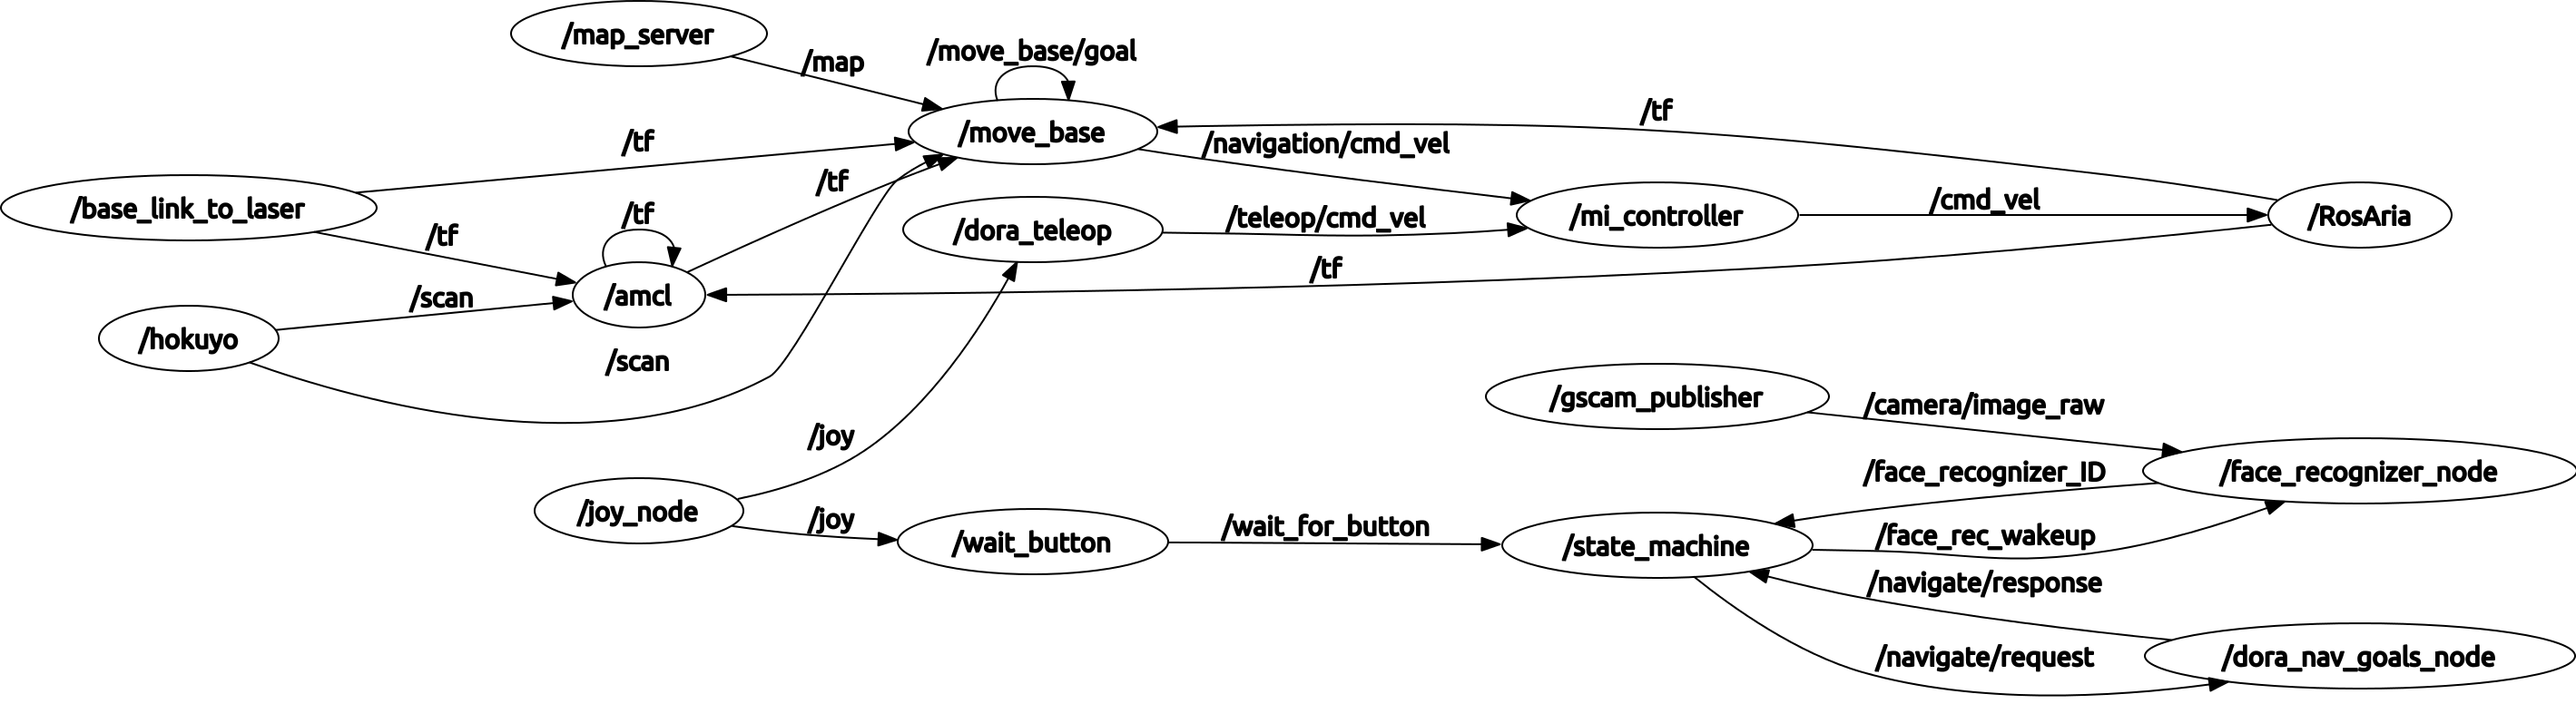
\includegraphics[width=\textwidth]{nodes_cut.png}
\caption{An overview of the software architecture and how the nodes connect and interact with each other}
\label{fig:nodes}
\end{figure*}

\subsection{State machine}
This year, we are focused on tasks, which can be easily defined as a sequence of some actions. Therefore, we decided to use a state machine as the control structure of our components. A state machine should generally monitor the state of a robot's components and switch between them according to predefined rules. Thus, it is the core element of our robotic system that connects the rest of the subsystems together.

For creating a state machine, we use ROS's SMACH package, that is ``a task-level architecture for rapidly creating complex robot behaviour" \cite{smach}. Our state machine can be seen in Fig. \ref{fig:smach} and it contains these states:
\begin{itemize}
\item Teleop - In order to perform the \textit{Welcoming visitors} task, a robot needs to recognise that someone is using the doorbell. This can be done by cooperating with an intelligent flat or by recognising a specific sound. However, we have not yet prepared any of these approaches. Therefore, we use a joystick as a simulation of pressing the doorbell. 
The second functionality of this state is to inform the robot that Dr. Kimbley has finished his work in Granny's bedroom. This state is only temporary, we will replace it with the recognition of a doorbell press and speech recognition for receiving a command from the doctor, respectively.
\item Navigate to a place - These states send navigation goal commands (see Section \ref{sec:navig}). For now, we have predefined the places in an existing map. However, we intend to extend this so that the robot will be able to find another correct position if a predefined place is occupied.
\item Speech - These states send a command with a predefined sentence to a speech synthesis node in order to improve the human interaction.
\item Face recognition - This state runs a node to detect a person at the front door, see Section \ref{sec:vision}.
\end{itemize}

Besides these nodes used in the state machine, we need additional functionalities such as building of a map, localisation, emergency stop and learning the face of the doctor. These and previous nodes are further described below.

\begin{figure}[!htb]
\centering
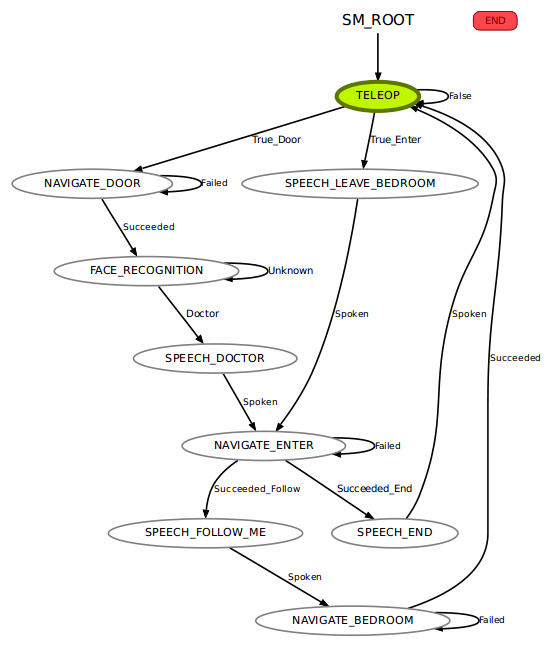
\includegraphics[width=3.in]{state_machine.png}
\caption{SMACH state machine connecting all subsystems to one robotic framework}
\label{fig:smach}
\end{figure}

\subsection{Building the map with SLAM}
According to the competition rules, it can be assumed that the robot can use a known map. In order to be able to create a map of the robot's environment, we used \textit{OpenSlam's GMapping} algorithm \cite{slam} through the ROS wrapper package called \textsf{slam gmapping}. This approach uses a Rao-Blackwellized particle filter in which each particle carries an individual map of the environment. The particles are updated by taking into account both odometry and the latest observations from a laser range finder.

\subsection{Localising in a known map with Adaptive Monte Carlo Localisation}
After the map is known and saved, an \textit{Adaptive Monte Carlo Localisation} (AMCL)\cite{amcl} algorithm is used to localise the robot inside the known environment. This node is part of the ROS \textsf{navigation stack} package. For details, see the section below. It uses laser range finder readings to update a particle filter. Every particle represents a specific discrete state and stores the uncertainty of the robot being in that state/position within the known map. Also, every time the robot moves it uses the motor information to shift the particles to the corresponding direction.

\subsection{\label{sec:navig}Navigation}
For navigation and obstacle avoidance, ROS's \textsf{navigation stack} is used. It is a proven robust solution for domestic environments \cite{Marder-Eppstein2010}. More specifically this node reads the odometry, the current pose estimate and the laser range finder scans from the relevant topics and safely drives the robot in the environment to a predefined goal. In order to navigate smoothly, it uses a combination of a global and a local planner. The global planner creates an optimal global path based on the robot's pose and a global cost-map. Then the local planner, which uses the \textit{Dynamic Window Approach} algorithm \cite{dwa}, is responsible for following the global path and reactively avoiding obstacles.

\subsection{Mixed initiative controller and teleoperation}
These nodes were made as part of another project involving mixed initiative HRI in emergency response robots. They allow switching between autonomous behaviour and teleoperation. Of course, this will not be used during the competition, but it is a helpful functionality during testing, when we can easily pause the robot's behaviour or place the robot in a specific position in its environment. Moreover, it provides a remote emergency stop, which increases the safety of the robot.

\subsection{\label{sec:vision}Face detection and recognition}
In order to be able to recognise a person standing in front of the entrance, the system implements face detection, which is used to find candidate face patterns inside an image, and face recognition, which finds the best match of a detected face with a known dataset, see Fig. \ref{fig:face}.

Face detection is performed using the \textit{Viola-Jones} algorithm \cite{Viola01_RapidObjDet}. The algorithm looks for faces by applying incrementally many simple Haar classifiers. The composition is performed by a cascade function, which needs to be trained \textit{a priori} with many positive and negative images. The resulting classifier can find faces efficiently with independence of the size of the faces and light conditions.

Face recognition is performed by applying a \textit{Local Binary Pattern Histogram} (LBPH) algorithm \cite{Ahonen04_FaceRecLBP}. The principle of the algorithm is to build local binary patterns (LBP) for each pixel depending on a variable neighbourhood scheme. Then, it divides the formed LBP image into $m$ local regions and computes the LBP distribution histogram from each region. Finally, classification is performed by comparison between the LBP histograms of a new face with the ones from the dataset.

\begin{figure}[!t]
\centering
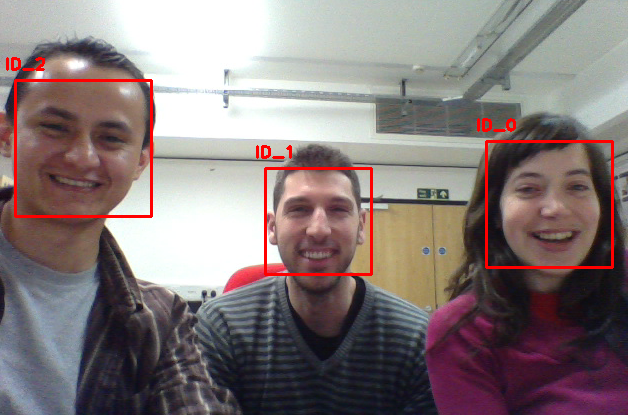
\includegraphics[width=3.in]{BARC_FaceRec.png}
\caption{An example of the face detection and face recognition algorithms. The red bounding boxes surround the successfully detected faces, while each of them is given a corresponding identification code.}
\label{fig:face}
\end{figure}


% An example of a floating figure using the graphicx package.
% Note that \label must occur AFTER (or within) \caption.
% For figures, \caption should occur after the \includegraphics.
% Note that IEEEtran v1.7 and later has special internal code that
% is designed to preserve the operation of \label within \caption
% even when the captionsoff option is in effect. However, because
% of issues like this, it may be the safest practice to put all your
% \label just after \caption rather than within \caption{}.
%
% Reminder: the "draftcls" or "draftclsnofoot", not "draft", class
% option should be used if it is desired that the figures are to be
% displayed while in draft mode.
%
%\begin{figure}[!t]
%\centering
%\includegraphics[width=2.5in]{myfigure}
% where an .eps filename suffix will be assumed under latex, 
% and a .pdf suffix will be assumed for pdflatex; or what has been declared
% via \DeclareGraphicsExtensions.
%\caption{Simulation Results}
%\label{fig_sim}
%\end{figure}

% Note that IEEE typically puts floats only at the top, even when this
% results in a large percentage of a column being occupied by floats.


% An example of a double column floating figure using two subfigures.
% (The subfig.sty package must be loaded for this to work.)
% The subfigure \label commands are set within each subfloat command, the
% \label for the overall figure must come after \caption.
% \hfil must be used as a separator to get equal spacing.
% The subfigure.sty package works much the same way, except \subfigure is
% used instead of \subfloat.
%
%\begin{figure*}[!t]
%\centerline{\subfloat[Case I]\includegraphics[width=2.5in]{subfigcase1}%
%\label{fig_first_case}}
%\hfil
%\subfloat[Case II]{\includegraphics[width=2.5in]{subfigcase2}%
%\label{fig_second_case}}}
%\caption{Simulation results}
%\label{fig_sim}
%\end{figure*}
%
% Note that often IEEE papers with subfigures do not employ subfigure
% captions (using the optional argument to \subfloat), but instead will
% reference/describe all of them (a), (b), etc., within the main caption.


% An example of a floating table. Note that, for IEEE style tables, the 
% \caption command should come BEFORE the table. Table text will default to
% \footnotesize as IEEE normally uses this smaller font for tables.
% The \label must come after \caption as always.
%
%\begin{table}[!t]
%% increase table row spacing, adjust to taste
%\renewcommand{\arraystretch}{1.3}
% if using array.sty, it might be a good idea to tweak the value of
% \extrarowheight as needed to properly center the text within the cells
%\caption{An Example of a Table}
%\label{table_example}
%\centering
%% Some packages, such as MDW tools, offer better commands for making tables
%% than the plain LaTeX2e tabular which is used here.
%\begin{tabular}{|c||c|}
%\hline
%One & Two\\
%\hline
%Three & Four\\
%\hline
%\end{tabular}
%\end{table}


% Note that IEEE does not put floats in the very first column - or typically
% anywhere on the first page for that matter. Also, in-text middle ("here")
% positioning is not used. Most IEEE journals/conferences use top floats
% exclusively. Note that, LaTeX2e, unlike IEEE journals/conferences, places
% footnotes above bottom floats. This can be corrected via the \fnbelowfloat
% command of the stfloats package.

\section{Conclusion}
%TODO proof reading
%from rules: Applicability and relevance to domestic/industrial robotics [@Home / @Work]
%Lenka
Our team has strong relevance to the domestic service robotics, as
Lenka's, Marco's and Manolis's research interests involved cooperation with
humans. We would like to use our expertises to combine the state of the art
in AI techniques with our own contributions. As a result, a robotic system
will be created with high reusability, as we use ROS middleware.

We would like to achieve high robustness of our robotic system that it can perform tasks repeatedly. In order of this our goal, we would like to put attention to verification and evaluation of our system. Therefore, we decided to focus only on a part of the RoCKIn@Home challenge this year. We expect that our robot Dora will be able to perform completely
the \textit{Welcoming visitors} task and recognise the doors' state in the
\textit{Getting to know my home} task. In order of fulfil these tasks, we
plan to merge techniques for face and an uniform detection, speech
recognition and synthesis, navigation, people detection, HRI behaviour that
will ensure that a person is following the robot, door detection, following
a person and gesture recognition.

Moreover, we plan to cooperate more with first year bachelor's students in
order to introduce them to robotics and provide them with some interesting
challenges, which can be used during competition. We believe that
participating in the RoCKIn@Home challenge will bring a lot of experience
not only to the young students, but also to us. As a result, we are
expecting to obtain more knowledge in the ongoing research in many fields
of robotics.

%All team members have research interests in areas where a robot must cooperate with people in order to provide the best performance. To summarize, Lenka is working on the STRANDS project, which aims to develop robots capable of helping elderly people with every day activities. Marco is interested in activity recognition which can significantly improve the cooperation of robots and humans. Manolis is doing research on flexible robotic control via cooperation between a human and an autonomous robot, especially in environments which are difficult for a robot. Sean did his bachelor's project on visual robot localisation in human crowds. Therefore, we believe that our work is strongly relevant to the RoCKIn@Home challenge.

%Moreover, if our team participates in this challenge, it will be an interesting challenge especially to newly incoming members, as we are expecting that more first year bachelor's students will join the team this summer. 



% conference papers do not normally have an appendix


% use section* for acknowledgement
%\section*{Acknowledgment}



% trigger a \newpage just before the given reference
% number - used to balance the columns on the last page
% adjust value as needed - may need to be readjusted if
% the document is modified later
%\IEEEtriggeratref{8}
% The "triggered" command can be changed if desired:
%\IEEEtriggercmd{\enlargethispage{-5in}}

% references section

% can use a bibliography generated by BibTeX as a .bbl file
% BibTeX documentation can be easily obtained at:
% http://www.ctan.org/tex-archive/biblio/bibtex/contrib/doc/
% The IEEEtran BibTeX style support page is at:
% http://www.michaelshell.org/tex/ieeetran/bibtex/


\bibliographystyle{IEEEtran}
\bibliography{./ref}
%
% <OR> manually copy in the resultant .bbl file
% set second argument of \begin to the number of references
% (used to reserve space for the reference number labels box)
%\begin{thebibliography}{1}

%\bibitem{IEEEhowto:kopka}
%H.~Kopka and P.~W. Daly, \emph{A Guide to \LaTeX}, 3rd~ed.\hskip 1em plus
%0.5em minus 0.4em\relax Harlow, England: Addison-Wesley, 1999.

%\end{thebibliography}




% that's all folks
\end{document}


